\chapter{数值实验}
在本章中,我们进行了几个经典的测试并展示了测试结果.
在时间的积分上,我们采用的是经典的四阶龙格库塔方法.
对于测试的输入,即球面的三角剖分,我们通过以下方式得到.

\begin{figure}[htb]
	\label{fig:getTRI}
	\centering
	\subfigure[初始三角网格]{
		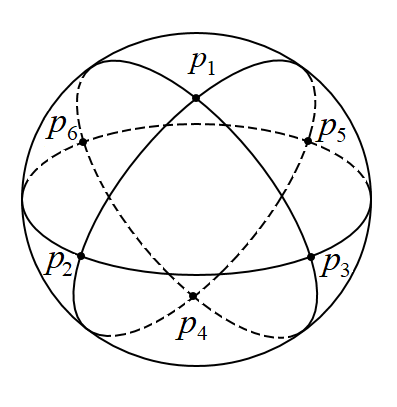
\includegraphics[width=0.4\linewidth]{images/ball}
	}
	\hfill
	\subfigure[对于初始三角网格的细化]{
		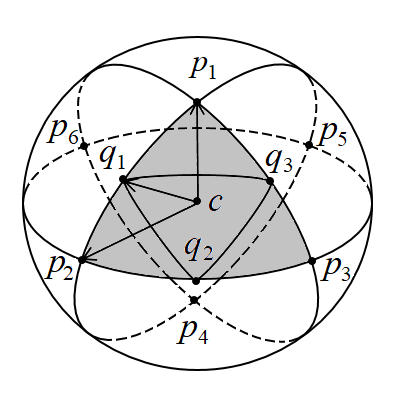
\includegraphics[width=0.4\linewidth]{images/ball3}
	}
	\caption{初始网格生成示意图}
\end{figure}

以球心是原点的单位球为例,在初始时刻给出所要剖分的球面的以下信息:
\begin{enumerate}
	\setlength{\itemsep}{0pt}
	\setlength{\parsep}{0pt}
	\setlength{\parskip}{0pt}
	\item 球心$c=(0,0,0)$,
	\item 半径$r=1$,
	\item 三角剖分信息(定义\ref{defn:triangulation}).
\end{enumerate}
三角剖分信息的给定不是唯一的,文中最初给定的三角剖分信息如下,见图4.1(a)
\begin{enumerate}
	\setlength{\itemsep}{0pt}
	\setlength{\parsep}{0pt}
	\setlength{\parskip}{0pt}
	\item 顶点个数$n_v=6$,三角形个数$n_t=8$;
	\item $6\times 3$的矩阵Pts,第$i$行表示了第$i$个顶点的坐标;
	\item $8\times 3$的矩阵,第$i$行的三个元素表示了第$i$个三角形的三个顶点在矩阵Pts中的指标.
\end{enumerate}
另外我们要求每个三角形的法向与其三个顶点满足右手法则,
并且所有三角形的法向朝球外部,这样做不仅利于计算多面体体积,
也为今后的殷集的布尔代数运算及样条曲面插值做铺垫.


在给出了初始的三角剖分之后,我们对其进行细化,
由于文中给出的初始三角剖分的每一个三角形都是正三角,
因此对于每个三角形我们都进行一致的细化操作.
以$p_1, p_2, p_3$所在的面为例,见图4.1(b).
已知球的球心为$c$,半径为$r$,则有

\begin{equation}
\left\{
\begin{array}{r}
\vec{cq_1}=r\cdot\frac{(\vec{cp_1}+\vec{cp_2})}{\|\vec{cp_1}+\vec{cp_2}\|},\\[0.2cm]
\vec{cq_2}=r\cdot\frac{(\vec{cp_2}+\vec{cp_3})}{\|\vec{cp_2}+\vec{cp_3}\|},\\[0.2cm]
\vec{cq_3}=r\cdot\frac{(\vec{cp_1}+\vec{cp_3})}{\|\vec{cp_1}+\vec{cp_3}\|}.\\[0.2cm]
\end{array}\right.
\end{equation}
$q_1, q_2, a_3$将$p_1, p_2, p_3$所在的三角曲面分割成四个三角曲面来达到初始网格的细化,
我们要求细化之后的网格依然满足右手法则,法向朝球外部.
通过对网格的多次细化来得到合适的球的三角剖分信息,
例如对初始三角剖分进行三次细化和四次细化得到了图4.2.

\begin{figure}[htb]
	\label{fig:refine}
	\centering
	\subfigure[初始网格进行三次细化之后的网格]{
		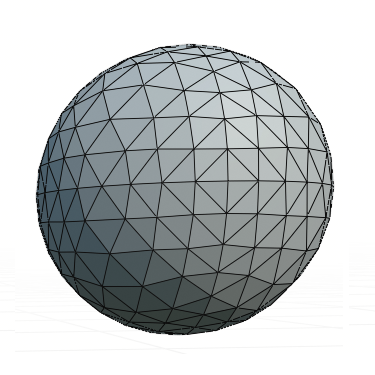
\includegraphics[width=0.4\linewidth]{images/3refine}
	}
	\hfill
	\subfigure[初始网格进行四次细化之后的网格]{
		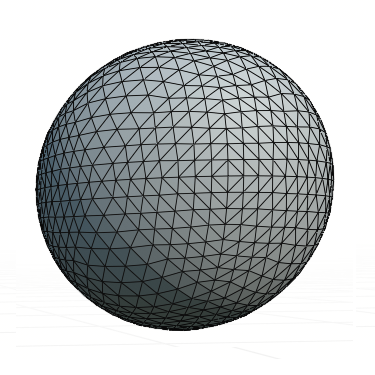
\includegraphics[width=0.4\linewidth]{images/4refine}
	}
	\caption{细化后的网格示意图}
\end{figure}


另外,由于直接求解1-范数\eqref{defn:error}较为困难,
在数值实验中,我们定义以下无穷范数和体积范数来作为准则,
\begin{equation}
E_{\infty}(T)=\max| r_i-r|.
\end{equation}
其中$r_i=\|p_i-C\|$,$p_i$是结束时刻所得流相界面的三角剖分上的顶点,
$C$是测试球的球心,$r$是测试球的半径.
\begin{equation}
E_{\mathrm{vol}}(T)=|V_{\mathrm{origin}}-V_{\mathrm{result}}|
\end{equation}
其中$V_{\mathrm{origin}}$是初始时刻用来近似流体的多面体体积,
$V_{\mathrm{result}}$是结束时刻所得的近似流体的多面体体积.



\section{二维剪切流场测试}
剪切流场中,$xy$方向上的流速由以下流函数给出,
\begin{equation*}
\psi (x,y)=-\frac{1}{\pi}\sin^2(\pi x)\sin^2(\pi y)\cos(\frac{\pi t}{T}),
\end{equation*}
而在$z$方向的速度为$0$, linear MARS在$\frac{T}{2}$时刻,
$x$和$y$方向上的流速符号被余弦项$\cos(\frac{\pi  t}{T})$反转,
因此在一个周期之后精确值与初始值完全一致,
测试参数见图\ref{tab:vortexSetup}.
在周期$T=8$的测试前半个阶段,
流相被速度场不断的拉伸变形成一个螺旋卷曲的薄片,
薄片向涡流中心旋转而存在被撕裂的可能.
这个测试中,尽管流体在几何上的形变很大,
但因流函数是同胚映射,流相不发生拓扑变化,
linear MARS方法良好的保持了剪切流场中流相的拓扑结构,
如图\ref{fig:vortexT8}.

\begin{figure}[htbp]
	\begin{minipage}[b]{0.65\linewidth}
		\renewcommand{\arraystretch}{1.2}
		\centering
		    \begin{tabular}{c|c}
      \hline
      参数名称 & 参数值  \\
      \hline
      测试区域     & $\Omega=[0,1]\times[0,1]\times[-0.5,0.5]$ \\
      测试时段 & $t\in[0,T]$ \\
      形状参数  & $C=(0.5,0.75,0.0)$, $R=0.15$ \\
      速度周期     & $T = 8$  \\
      库朗数 & $\text{Cr}=1$               \\
      控制体网格大小
      & $h = \frac{1}{16}, \frac{1}{32}, \frac{1}{64},  \frac{1}{128}$  \\
      界面尺度
      & $h_L= O(h), O(h^{\frac{3}{2}}), O(h^2)$, $r_{\mathsf{tiny}}=0.01$
      \\
      \hline
      \multicolumn{2}{c}{}\\
    \end{tabular}

%%% Local Variables: 
%%% mode: latex
%%% TeX-master: "../cubicMARS"
%%% End: 

	\end{minipage}
	\hfill
	\begin{minipage}{0.3\linewidth}
		\centering
		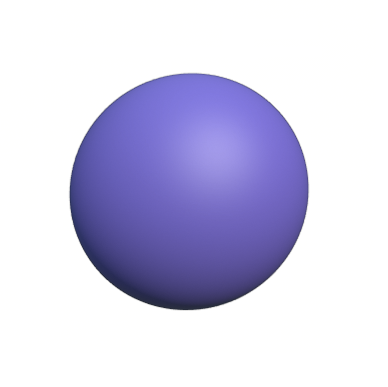
\includegraphics[width=1\linewidth]{images/3}
	\end{minipage}
	\caption{二维剪切流场测试参数}
	\label{tab:vortexSetup}
\end{figure}



\begin{figure}[htbp]
	\centering
	\subfigure[$t=0$]{
		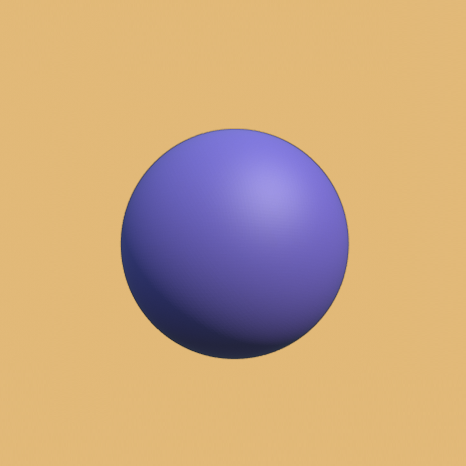
\includegraphics[width=0.305\linewidth]{images/v1}
	}
	\hfill
	\subfigure[$t=\frac{1}{8}T$]{
		
\includegraphics[width=0.305\linewidth]{images/v2}
	}
	\hfill
	\subfigure[$t=\frac{1}{4}T$]{
		
\includegraphics[width=0.305\linewidth]{images/v3}
	}
	
	\subfigure[$t=\frac{1}{2}T$]{
		
\includegraphics[width=0.30\linewidth]{images/v4}
	}
	\hfill
	\subfigure[$t=\frac{3}{4}T$]{
		
\includegraphics[width=0.305\linewidth]{images/v5}
	}
	\hfill
	\subfigure[$t=T$]{
		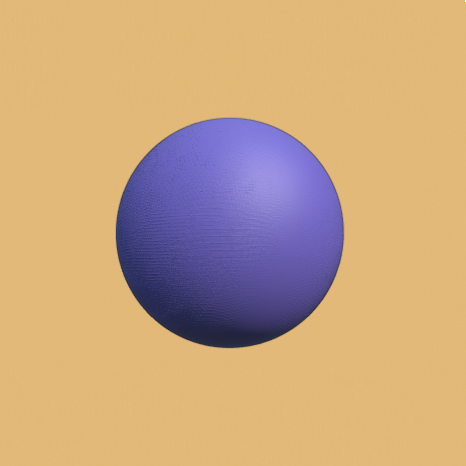
\includegraphics[width=0.305\linewidth]{images/v6}
	}
	\caption[二维剪切流场测试结果]{$T=8,r_{\mathsf{tiny}}=0.01,h_L=1/128$时,
		二维剪切流场的测试结果图.$(n_v,n_t)$在$T=0, \frac{T}{2}, T$时刻的值分别是$(16386,32768)$,$(272023,544042)$和$(166696,333388)$,
		$t=T$时刻的误差$E_{\infty}=4.11e-04,E_{\mathrm{vol}}=1.34e-06$.}
	\label{fig:vortexT8}
\end{figure}

%\begin{table}[htbp]
%	\label{tab1}
%	\centering
%	\caption[二维剪切流场的误差测试结果]{当$r_{\mathrm{tiny}}=0.01$时,二维剪切流场测试的误差结果}
%	\begin{tabular}{c|ccccccc}
%		\hline \hline
%		%    \multicolumn{2}{c|}{\rule[-3mm]{0mm}{8mm} Methods }
%		%Methods
%		&$h=\frac{1}{16}$ & rate & $h=\frac{1}{32}$ 
%		& rate & $h=\frac{1}{64}$ & rate &  $h=\frac{1}{128}$
%		\\ \hline 
%		& \multicolumn{6}{c}{$T=2$ }
%		\\ \hline 
%		$h_L=0.5h,E_{\infty}$ & 1.15e-03 & 1.91 & 3.05e-04 & 1.88&8.30e-05 & 2.05 & 2.00e-05
%		\\
%		$h_L=0.5h,E_{\mathrm{vol}}$  & 4.31e-06 & 1.92 & 1.14e-06 & 1.84 &3.18e-07 & 1.94 & 8.26e-08
%		\\ \hline 
%		$h_L=8h^{\frac{3}{2}},E_{\infty}$ & - & -  & 3.42e-03 & 2.77& 5.03e-04 & 3.13 & 5.73e-05
%		\\
%		$h_L=8h^{\frac{3}{2}},E_{\mathrm{vol}}$  & - & - & 2.70e-05 & 4.39 &1.29e-06& 2.46 & 2.34e-07
%		\\ \hline 
%		$h_L=64h^2,E_{\infty}$ & - & - & 2.78e-03 & 3.19 &3.05e-04 & 3.93 & 2.00e-05
%		\\
%		$h_L=64h^2,E_{vol}$  & - & - & 1.05e-05 & 3.02 &1.29e-06 & 3.97 & 8.26e-08
%		\\ \hline 
%		& \multicolumn{6}{c}{$T=4$ }
%		\\ \hline 
%		$h_L=0.5h,E_{\infty}$ & 1.74e-03 & 2.00 & 6.96e-04 & 2.00 &1.74e-04 & 2.00 & 4.36e-05
%		\\
%		$h_L=0.5h,E_{vol}$  & 1.18e-05 & 1.99 & 3.20e-06 & 2.07 &7.61e-07 & 2.00 & 1.90e-07
%		\\ \hline 
%		$h_L=8h^{\frac{3}{2}},E_{\infty}$ & - & - & 5.93e-03 & 3.09 &6.95e-04 & 2.90 & 9.30e-05
%		\\
%		$h_L=8h^{\frac{3}{2}},E_{\mathrm{vol}}$  & - & - & 4.51e-05 & 3.75 &00e-00 & 2.69 & 4.92e-07
%		\\ \hline 
%		$h_L=64h^2,E_{\infty}$ & - & - & 1.20e-02 & 4.11 &6.95e-04 & 3.99 & 4.36e-05
%		\\
%		$h_L=64h^2,E_{vol}$  & - & - & 5.78e-05 & 4.2 &3.14e-06 & 4.06 & 1.88e-07
%		\\ \hline 
%		& \multicolumn{6}{c}{$T=8$ }
%		\\ \hline 
%		$h_L=0.5h,E_{\infty}$ & 6.46e-03 & 2.00 & 1.62e-03 & 1.98 &4.11e-04 & 2.01 & 1.02e-04
%		\\
%		$h_L=0.5h,E_{vol}$   & 1.96e-05 & 2.15 & 4.43e-06 & 1.72 &1.34e-06 & 2.08 & 3.17e-07
%		\\ \hline 
%		$h_L=8h^{\frac{3}{2}},E_{\infty}$ & - & - & 1.41e-02 & 3.46 &1.28e-03 & 2.89 & 1.72e-04
%		\\
%		$h_L=8h^{\frac{3}{2}},E_{\mathrm{vol}}$ &- & - & 5.77e-05 & 3.64 &4.63e-06 & 2.14 & 1.05e-06
%		\\ \hline 
%		$h_L=64h^2,E_{\infty}$ & - & - & 2.66e-04 & 4.04 &1.62e-03 & 3.98 & 1.03e-04
%		\\
%		$h_L=64h^2,E_{vol}$  & - & - & 7.01e-05 & 3.92 &4.63e-06 & 3.87 & 3.17e-07
%		\\ \hline \hline
%	\end{tabular}
%\end{table}  

\begin{table}[htbp]
	\label{tab1}
	\centering
	\caption[二维剪切流场测试的误差结果]{当$r_{\mathsf{tiny}}=0.01$时,二维剪切流场测试的误差结果}
	\begin{tabular}{c|ccccccc}
		\hline \hline
		%    \multicolumn{2}{c|}{\rule[-3mm]{0mm}{8mm} Methods }
		%Methods
		&$h=\frac{1}{16}$ & rate & $h=\frac{1}{32}$ 
		& rate & $h=\frac{1}{64}$ & rate &  $h=\frac{1}{128}$
		\\ \hline 
		$h_L=0.5h,E_{\infty}$ & 6.46e-03 & 2.00 & 1.62e-03 & 1.98 &4.11e-04 & 2.01 & 1.02e-04
		\\
		$h_L=0.5h,E_{vol}$   & 1.96e-05 & 2.15 & 4.43e-06 & 1.72 &1.34e-06 & 2.08 & 3.17e-07
		\\ \hline 
		$h_L=8h^{\frac{3}{2}},E_{\infty}$ & - & - & 1.41e-02 & 3.46 &1.28e-03 & 2.89 & 1.72e-04
		\\
		$h_L=8h^{\frac{3}{2}},E_{\mathrm{vol}}$ &- & - & 5.77e-05 & 3.64 &4.63e-06 & 2.14 & 1.05e-06
		\\ \hline 
		$h_L=64h^2,E_{\infty}$ & - & - & 2.47e-04 & 3.93 &1.62e-03 & 3.99 & 1.02e-04
		\\
		$h_L=64h^2,E_{vol}$  & - & - & 7.01e-05 & 3.92 &4.63e-06 & 3.87 & 3.17e-07
		\\ \hline \hline
	\end{tabular}
\end{table}  

基于误差范数$E_{\infty}$和$E_{\mathrm{vol}}$,当$\alpha $分别取$1, \frac{3}{2}, 2$时,linear MARS方法基本上呈现了二、三、四阶精度,见表\ref{tab1}.
%在剪切流场的测试中,周期越长,流体的形变也就越大.从表$\ref{tab1}$中可得,当网格大小相同时,流相的形变越小,最终的误差$E_{\infty}$和$E_{\mathrm{vol}}$也越小.另外,基于误差范数$E_{\infty}$和$E_{\mathrm{vol}}$,当$\alpha $分别取$1, \frac{3}{2}, 2$时,linear MARS方法基本上呈现了二、三、四阶精度,见表\ref{tab1}.
\newpage

\section{二维变形流场测试}
变形流场测试被认为是界面追踪中最困难的问题之一.
其在$xy$方向上的流速由以下流函数得出,
\begin{equation*}
\label{eq:deformation}
\psi(x,y)=\frac{1}{n_{\mathrm{v}} \pi}\sin(n_{\mathrm{v}}(x+0.5))\cos(n_{\mathrm{v}}\pi(y+0.5))\cos(\frac{\pi t}{T}),
\end{equation*}
在$z$方向上的流速为$0$, $n_{\mathrm{v}}$表示在计算域中的涡流数,
流速符号在$\frac{T}{2}$时刻被余弦项$\cos(\frac{\pi  t}{T})$反转,
结束时刻其精确值与初始时刻一致,测试参数见图\ref{tab:deformation}.
在测试前半个周期中,流相的多个局部区域被流速场拉伸的很薄,
而linear MARS始终保持了流相的拓扑结构,如图\ref{fig:deformation}.
\begin{figure}[htbp]
	\begin{minipage}[b]{0.65\linewidth}
		\renewcommand{\arraystretch}{1.2}
		\centering
		    \begin{tabular}{c|c}
      \hline
      参数名称 & 参数值  \\
      \hline
      测试区域     & $\Omega=[0,1]\times[0,1]\times[-0.5,0.5]$ \\
      测试时段 & $t\in[0,T]$ \\
      形状参数  & $C=(0.5,0.5,0.0)$, $R=0.15$ \\
      速度参数    & $T = 2,n_{\mathrm{v}}=4$  \\
      库朗数 & $\text{Cr}=1$               \\
      控制体网格大小
      & $h = \frac{1}{16}, \frac{1}{32},\frac{1}{64},\frac{1}{128}$  \\
      界面尺度
      & $h_L= O(h), O(h^{\frac{3}{2}}), O(h^2)$, $r_{\mathsf{tiny}}=0.01$
      \\
      \hline
      \multicolumn{2}{c}{}\\
    \end{tabular}

%%% Local Variables: 
%%% mode: latex
%%% TeX-master: "../cubicMARS"
%%% End: 

	\end{minipage}
	\hfill
	\begin{minipage}{0.3\linewidth}
		\centering
		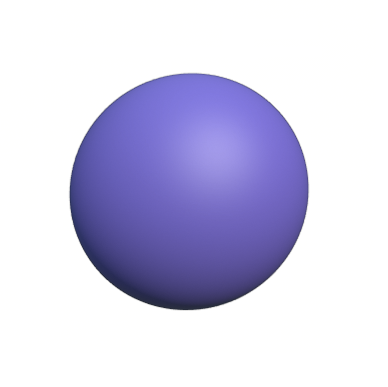
\includegraphics[width=1\linewidth]{images/3}
	\end{minipage}
	\caption{二维变形流场测试参数}
	\label{tab:deformation}
\end{figure}


\begin{figure}[htbp]
	\centering
	\subfigure[$t=0$]{
      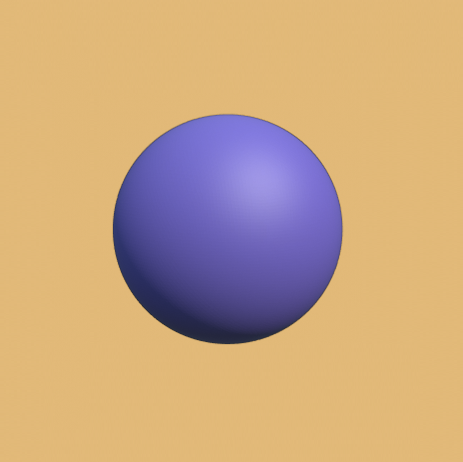
\includegraphics[width=0.315\linewidth]{images/d1}
	}
	\hfill
	\subfigure[$t=\frac{1}{8}T$]{
	  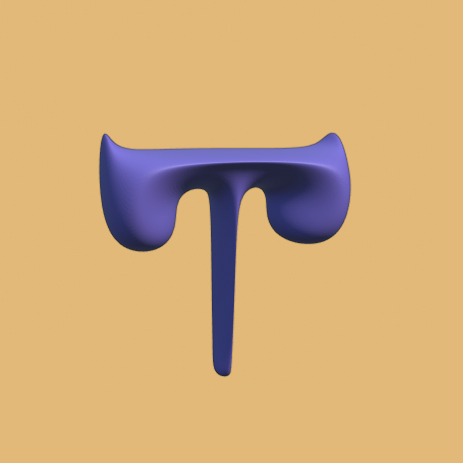
\includegraphics[width=0.315\linewidth]{images/d2}
	}
	\hfill
	\subfigure[$t=\frac{2}{8}T$]{
	  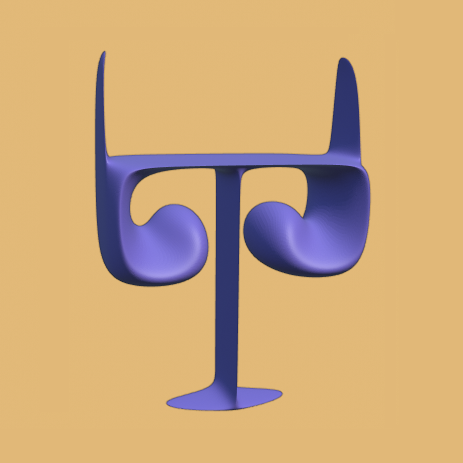
\includegraphics[width=0.315\linewidth]{images/d3}
	}
	
	\subfigure[$t=\frac{3}{8}T$]{
	  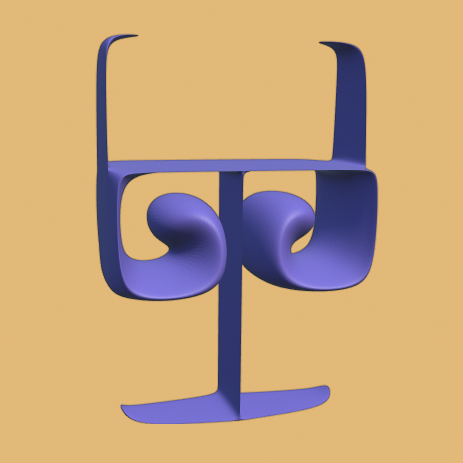
\includegraphics[width=0.315\linewidth]{images/d4}
	}
	\hfill
	\subfigure[$t=\frac{4}{8}T$]{
	  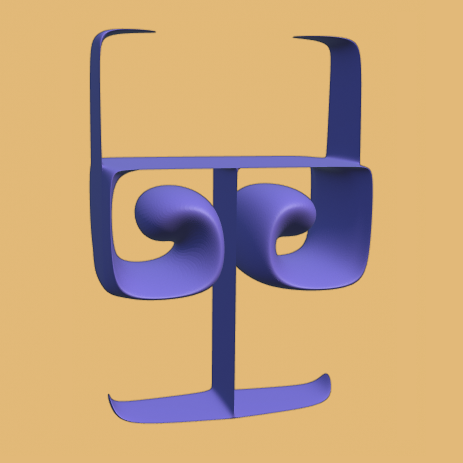
\includegraphics[width=0.315\linewidth]{images/d5}
	}
	\hfill
	\subfigure[$t=\frac{5}{8}T$]{
	  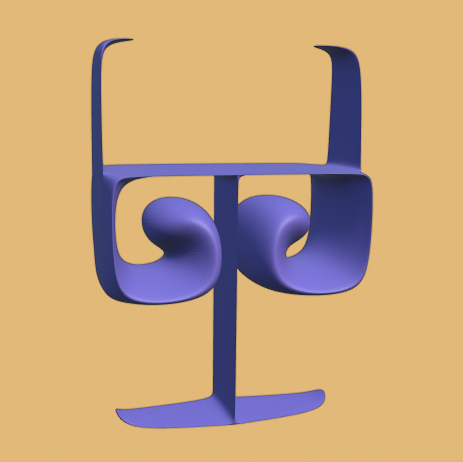
\includegraphics[width=0.315\linewidth]{images/d6}
	}
  	
  \subfigure[$t=\frac{6}{8}T$]{
  	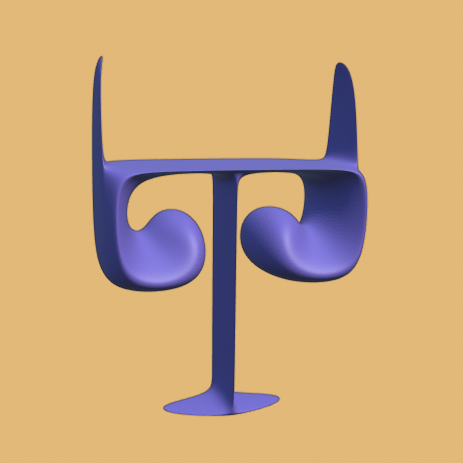
\includegraphics[width=0.315\linewidth ]{images/d7}
  }
  \hfill
  \subfigure[$t=\frac{7}{8}T$]{
   	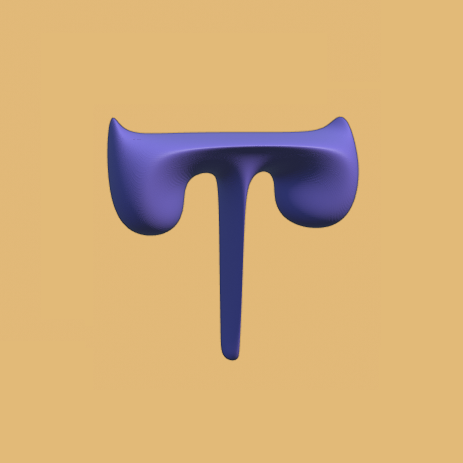
\includegraphics[width=0.315\linewidth ]{images/d8}
  }
  \hfill
  \subfigure[$t=T$]{
  	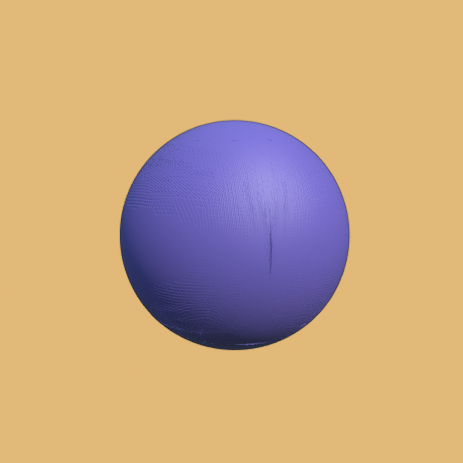
\includegraphics[width=0.315\linewidth ]{images/d9}
  }
	\caption[二维变形流场测试结果]{$T=2,n_{\mathrm{v}}=4,r_{\mathsf{tiny}}=0.01,h_L=1/128$时,
		二维变形流场的测试结果图.$(n_v,v_t)$在$T=0, \frac{T}{2}, T$时刻的值分别是$(16386,32768)$,$(444236,888468)$和$(116147,232290)$,
		$t=T$时刻的误差$E_{\infty}=5.81e-04,E_{\mathrm{vol}}=5.39e-07$.}
	\label{fig:deformation}
\end{figure}


\begin{table}[htb]
	\label{tab2}
	\centering
	\caption[二维变形流场测试的误差结果]{当$r_{\mathsf{tiny}}=0.01$时,二维变形流场测试的误差结果}
	\begin{tabular}{c|ccccccc}
		\hline \hline
		%    \multicolumn{2}{c|}{\rule[-3mm]{0mm}{8mm} Methods }
		linear MARS
		&$h=\frac{1}{16}$ & rate & $h=\frac{1}{32}$ 
		& rate & $h=\frac{1}{64}$ & rate &  $h=\frac{1}{128}$
		\\ \hline 
		& \multicolumn{6}{c}{$T=2,v_{\mathrm{v}}=4$ }
		\\ \hline 
		$h_L=h,E_{\infty}$ & 3.12e-02 & 1.93 & 8.16e-03 & 2.01 &2.03e-03 & 1.80& 5.81e-04
		\\
		$h_L=h,E_{\mathrm{vol}}$  & 2.42e-05 & 1.56 & 8.18e-06 & 1.63 &2.64e-06 & 2.29 & 5.39e-07
		\\ \hline 
		$h_L=8h^{\frac{3}{2}},E_{\infty}$ & - & - & 1.40e-02 & 2.79 & 2.03ee-03 & 2.57 & 3.43e-04
		\\
		$h_L=8h^{\frac{3}{2}},E_{\mathrm{vol}}$  & - & - & 8.93e-06 & 2.55 &1.53e-06 & 4.16 & 8.55e-08
		\\ \hline 
		$h_L=64h^2,E_{\infty}$ & - & - & 3.10e-02 &3.93 &2.03e-03 & 2.94 & 2.65e-04
		\\
		$h_L=64h^2,E_{\mathrm{vol}}$  & - & - & 2.69e-05 & 3.90 &1.80e-06 & 4.01 & 1.12e-07
		\\ \hline \hline
	\end{tabular}
\end{table}  

变形流场测试中,基于误差范数$E_{\infty}$和$E_{\mathrm{vol}}$,
当$\alpha$分别取$1,\frac{3}{2},2$时,linear MARS总体上呈现了二、三、四精度,
但也存在着个别测试没有达到理论精度.
这可能是由于流相在测试中的形变过大,造成了精度的降低,见表\ref{tab2}.


\section{三维剪切流场测试}
LeVeque\cite{leveque96}通过叠加$xy$平面上的形变与$xz$平面上的形变,
将二维的剪切流场扩展到了三维,提出了一个在三维空间中的不可压流场,
其三个方向的流速如下:
\begin{equation*}\label{bilevel}
\left\{\begin{array}{l}
v_x(x,y,z,t)=\cos(\frac{\pi  t}{T})2\sin^2(\pi x)\sin(2\pi y)\sin(2\pi z),\\[0.2cm]
v_y(x,y,z,t)=-\cos(\frac{\pi t}{T})\sin(2\pi x)\sin^2(\pi y)\sin(2 \pi z),\\[0.2cm]
v_z(x,y,z,t)=-\cos(\frac{\pi t}{T})\sin(2\pi x)\sin(2\pi y)\sin^2(\pi z).\\[0.2cm]
\end{array}\right.
\end{equation*}


流体的运动周期依赖于$\cos(\frac{\pi t}{T})$这一项.
同样的,流相在$\frac{T}{2}$时刻反转,
因此其在周期结束时刻恢复初始值,测试参数见图\ref{tab:de3}.
在测试的前半个周期,
球体被两个旋转的涡流夹带,
漩涡从两个相反方向作用于球体两侧,
并且挤压球体,
使球体变得很薄且形变后的流体两端变得十分伸展,
见图\ref{fig:3Dflow}.
LS方法对于处理这样的薄的界面追踪时,
最终结果可能改变流相的拓扑结构\cite{enright02:_hybrid_partic_level_set_method},
而linear MARS方法很好的保持了流相的拓扑信息.
\begin{figure}[htbp]
	\begin{minipage}[b]{0.65\linewidth}
		\renewcommand{\arraystretch}{1.2}
		\centering
		    \begin{tabular}{c|c}
      \hline
      参数名称 & 参数值  \\
      \hline
      测试区域     & $\Omega=[0,1]\times[0,1]\times[-0.5,0.5]$ \\
      测试时段 & $t\in[0,T]$ \\
      形状参数  & $C=(0.35,0.35,0.35)$, $R=0.15$ \\
      速度参数    & $T = 3$\\
      库朗数 & $\text{Cr}=1$               \\
      控制体网格大小
      & $h =  \frac{1}{16}, \frac{1}{32}, \frac{1}{64}, \frac{1}{128}$  \\
      界面尺度
      & $h_L= O(h), O(h^{\frac{3}{2}}),O(h^2)$, $r_{\mathrm{tiny}}=0.01,0.1$
      \\
      \hline
      \multicolumn{2}{c}{}\\
    \end{tabular}

%%% Local Variables: 
%%% mode: latex
%%% TeX-master: "../cubicMARS"
%%% End: 

	\end{minipage}
	\hfill
	\begin{minipage}{0.3\linewidth}
		\centering
		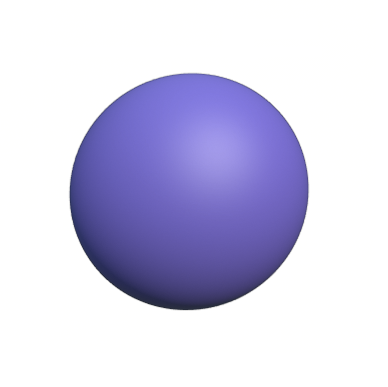
\includegraphics[width=1\linewidth]{images/3}
	\end{minipage}
	\caption{三维剪切流场测试参数}
	\label{tab:de3}
\end{figure}
%\begin{figure}
%	\label{fig:de3}
%	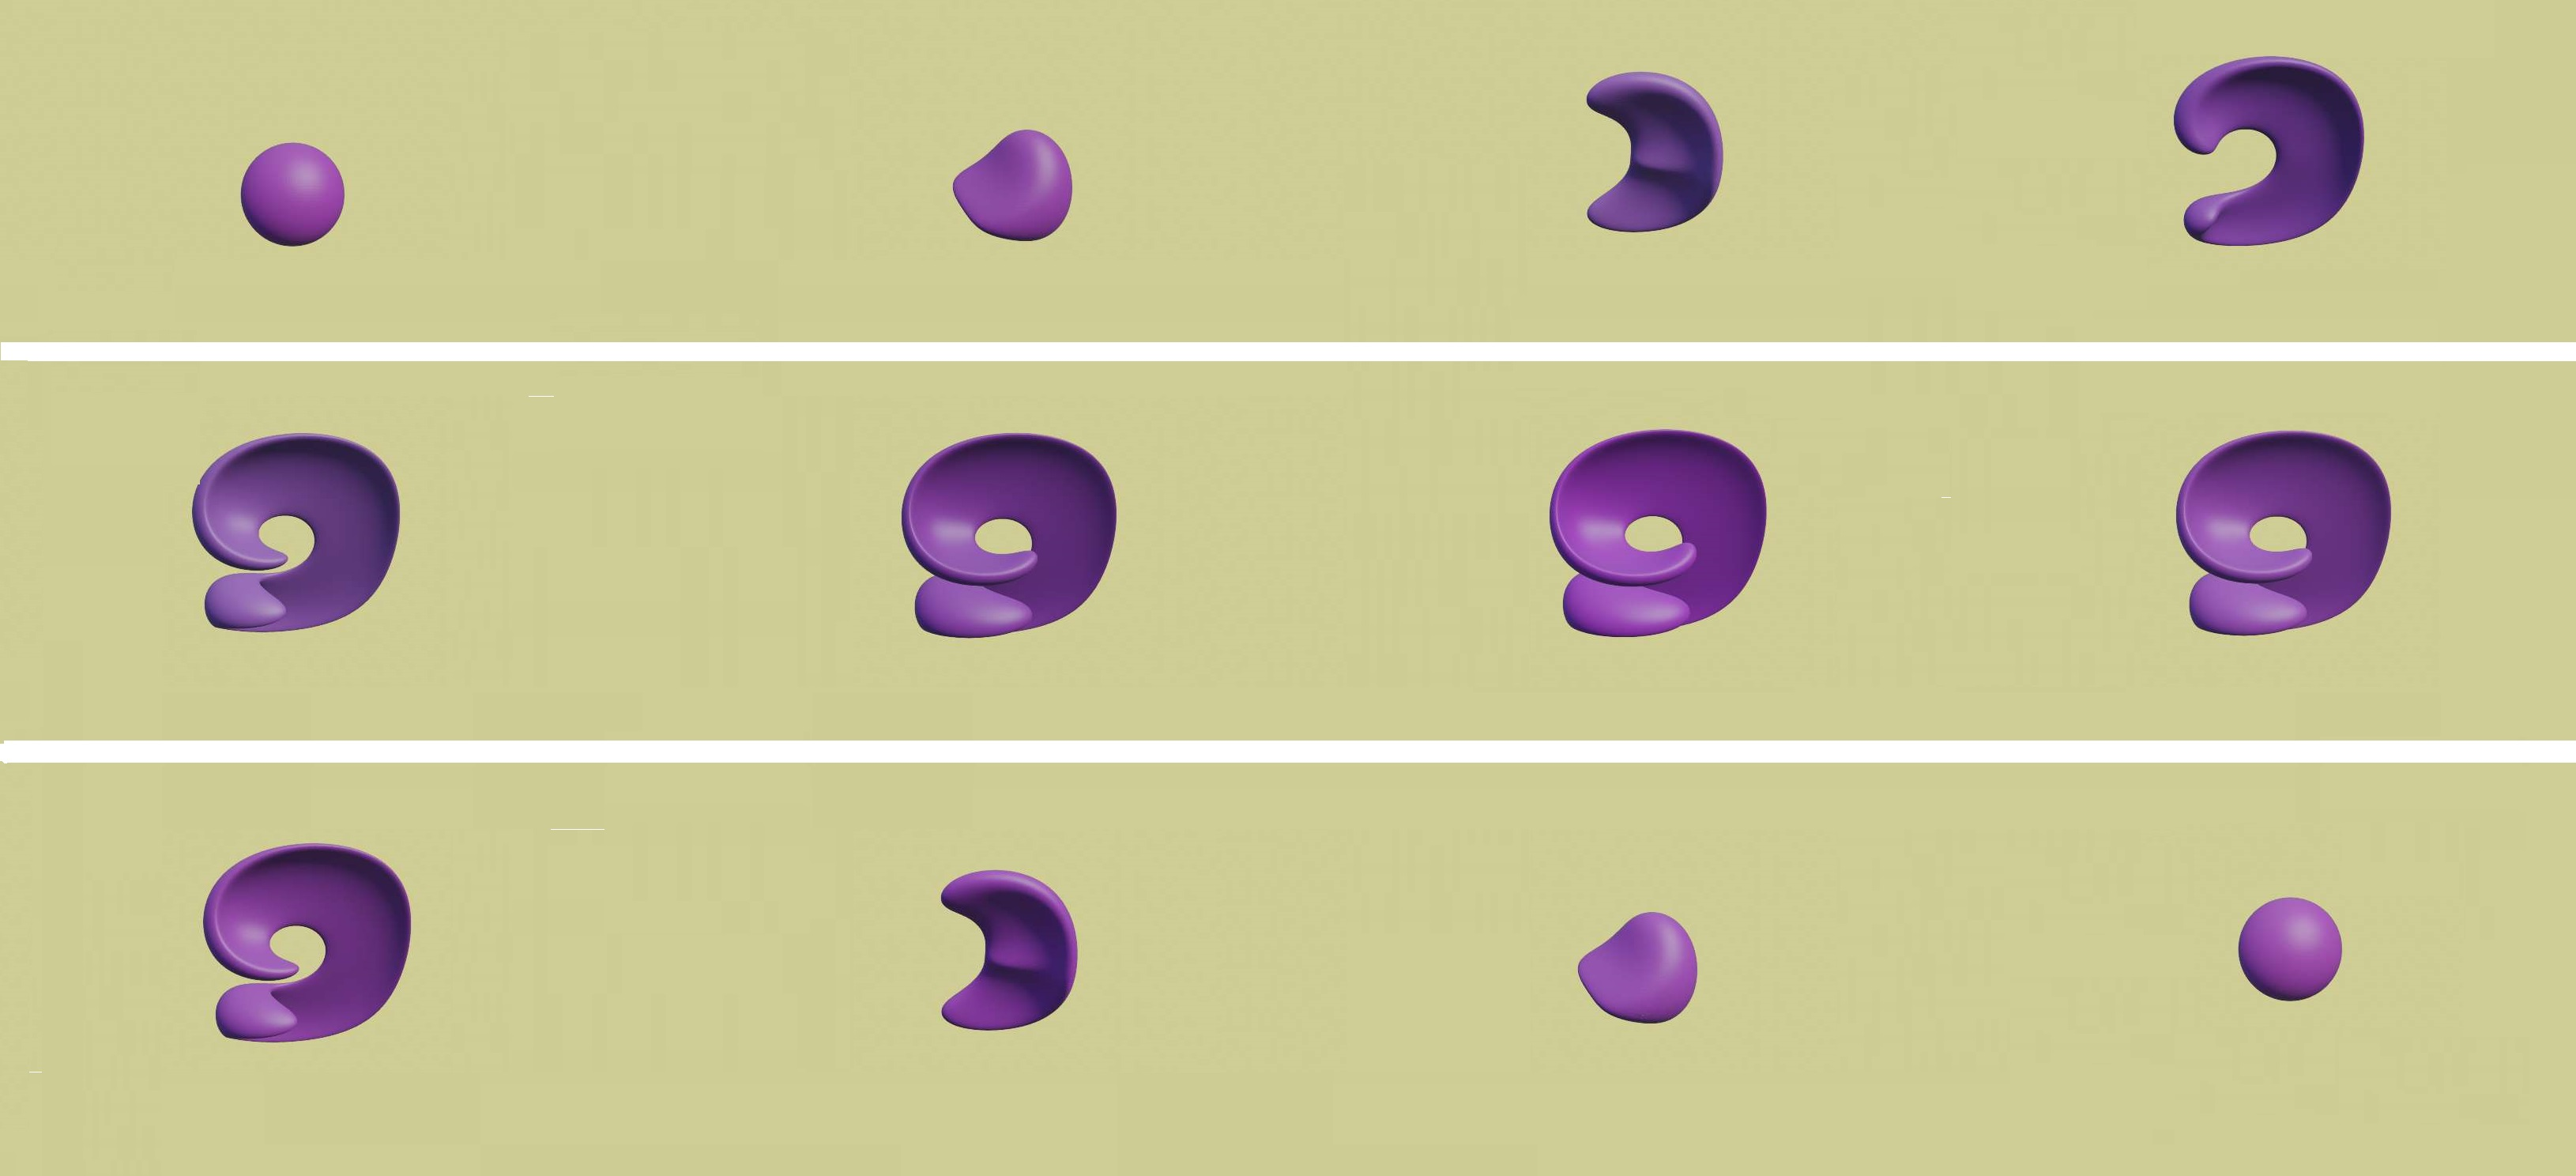
\includegraphics[width=\linewidth]{images/三维渲染图}
%	\caption[三维变形流场测试结果]{$h_L=1/128$时,三维变形流场测试中流相的形变过程图}
%\end{figure}

\begin{table}[htbp]
	\label{tab3}
	\centering
	\caption[$r_{\mathsf{tiny}}=0.01$时,三维剪切流场测试的误差结果]{当$r_{\mathsf{tiny}}=0.01$时,
		三维变形流场测试的误差结果}
	\begin{tabular}{c|ccccccc}
		\hline \hline
		%    \multicolumn{2}{c|}{\rule[-3mm]{0mm}{8mm} Methods }
		linear MARS
		&$h=\frac{1}{16}$ & rate & $h=\frac{1}{32}$ 
		& rate & $h=\frac{1}{64}$ & rate &  $h=\frac{1}{128}$
		\\ \hline 
		$h_L=0.5h,E_{\infty}$ & 6.03e-03 & 2.21 & 1.30e-03 & 2.10 &3.03e-04 & 1.95 & 7.85e-05
		\\
		$h_L=0.5h,E_{\mathrm{vol}}$  & 2.97e-05 & 2.65 & 4.73e-06 & 2.09 &1.12e-06 & 1.87 & 3.06e-07
		\\ \hline 
		$h_L=8h^{\frac{3}{2}},E_{\infty}$ & - & - & 1.00e-02 & 2.95 &1.29e-03 & 3.26 & 1.35e-04
		\\
		$h_L=8h^{\frac{3}{2}},E_{\mathrm{vol}}$  & - & - & 7.08e-05 & 3.72 &5.39e-06 & 3.25 & 5.67e-07
		\\ \hline 
		$h_L=64h^2,E_{\infty}$ & - & - & 2.62e-02 & 4.33 &1.30e-03 & 4.05 & 7.85e-05
		\\
		$h_L=64h^2,E_{\mathrm{vol}}$  & - & - & 9.27e-05 & 4.10 &5.39e-06 & 4.14 & 3.06e-07
		\\ \hline \hline
	\end{tabular}
\end{table}  

\begin{table}[htbp]
	\label{tab4}
	\centering
		\caption[$r_{\mathsf{tiny}}=0.1$时,三维剪切流场测试的误差结果]{当$r_{\mathsf{tiny}}=0.1$时,
			三维剪切流场测试的误差结果}
	\begin{tabular}{c|ccccccc}
		\hline \hline
		%    \multicolumn{2}{c|}{\rule[-3mm]{0mm}{8mm} Methods }
		linear MARS
		&$h=\frac{1}{16}$ & rate & $h=\frac{1}{32}$ 
		& rate & $h=\frac{1}{64}$ & rate &  $h=\frac{1}{128}$
		\\ \hline 
		$h_L=0.5h,E_{\infty}$ & 1.96e-02 & 2.19 & 4.30e-03 &1.53&1.49e-03& 1.33 & 5.93e-04
		\\
		$h_L=0.5h,E_{\mathrm{vol}}$  & 3.05e-04 & 1.90 & 8.17e-05 & 1.87 &2.23e-05 & 1.93 & 5.86e-06
		\\ \hline 
		$h_L=8h^{\frac{3}{2}},E_{\infty}$ & - & - & 3.69e-02 & 3.13 &4.21e-03 & 2.11 & 9.76e-04
		\\
		$h_L=8h^{\frac{3}{2}},E_{\mathrm{vol}}$  & - & - & 5.14e-04 & 2.59&8.53e-05 & 2.83 & 1.20e-05
		\\ \hline 
		$h_L=64h^2,E_{\infty}$ & - & - & 6.02e-02 & 3.84 &4.21e-03 & 2.83 & 5.93e-04
		\\
		$h_L=64h^2,E_{\mathrm{vol}}$  & - & - & 9.44e-04 & 3.44 &8.70e-05 & 3.88 & 5.89e-06
		\\ \hline \hline
	\end{tabular}
\end{table}  

三维变形流场测试中,基于误差范数$E_{\infty}$和$E_{\mathrm{vol}}$,
当$r_{\mathsf{tiny}}=0.01$,$\alpha$分别取值$1,\frac{3}{2},2$时,
linear MARS方法分别呈现出了二、三、四阶精度,见表\ref{tab3}.
当$r_{\mathsf{tiny}}=0.1$时,
测试的运行时间降低,而最终的误差有所加大,
同时精度也有所下降,见表\ref{tab4}.

\begin{figure}[htbp]
	\centering
	\subfigure[$t=0$]{
		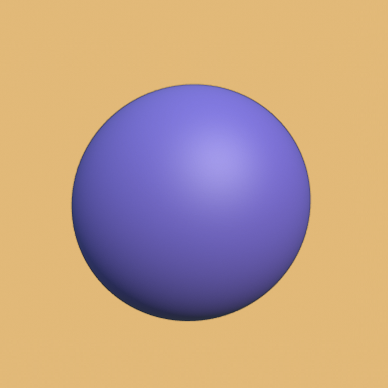
\includegraphics[width=0.3\linewidth]{images/3d-1}
	}
	\hfill
	\subfigure[$t=\frac{1}{8}T$]{
		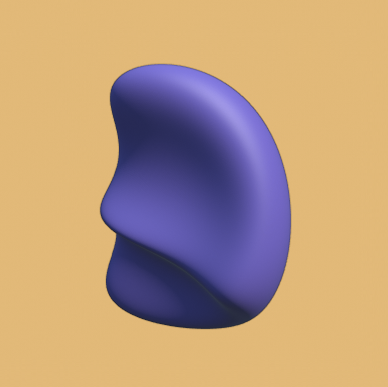
\includegraphics[width=0.3\linewidth]{images/3d-2}
	}
	\hfill
	\subfigure[$t=\frac{2}{8}T$]{
		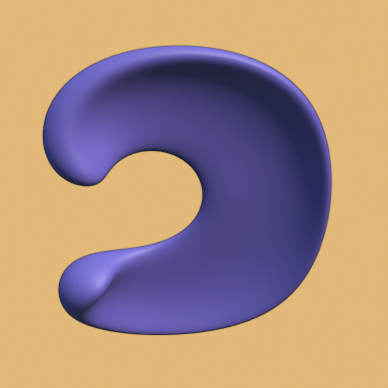
\includegraphics[width=0.3\linewidth]{images/3d-3}
	}
	
	\subfigure[$t=\frac{3}{8}T$]{
		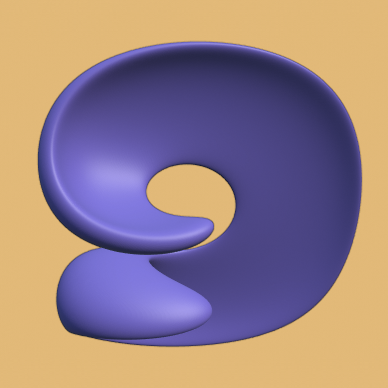
\includegraphics[width=0.3\linewidth]{images/3d-4}
	}
	\hfill
	\subfigure[$t=\frac{4}{8}T$]{
		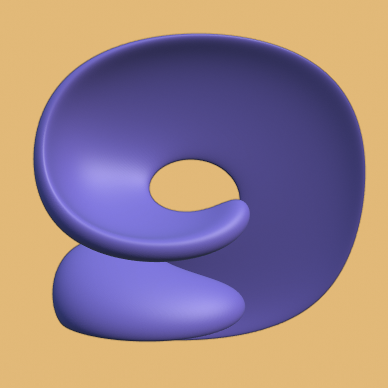
\includegraphics[width=0.3\linewidth]{images/3d-5}
	}
	\hfill
	\subfigure[$t=\frac{5}{8}$]{
		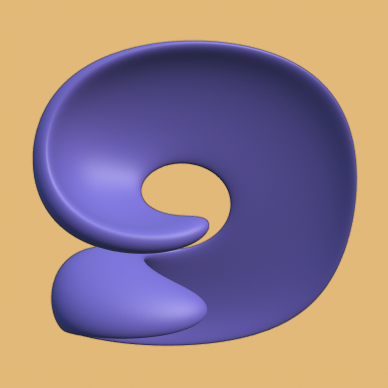
\includegraphics[width=0.3\linewidth]{images/3d-6}
	}
	
	\subfigure[$t=\frac{6}{8}T$]{
		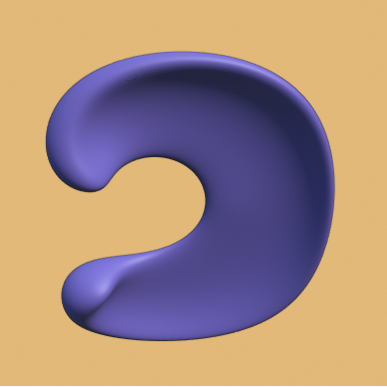
\includegraphics[width=0.3\linewidth ]{images/3d-7}
	}
	\hfill
	\subfigure[$t=\frac{7}{8}T$]{
		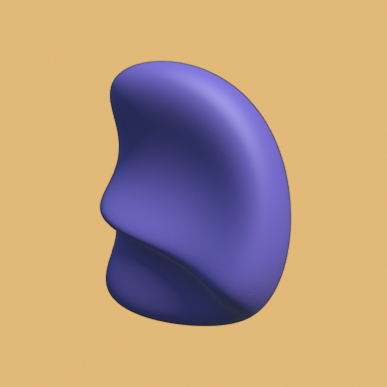
\includegraphics[width=0.3\linewidth ]{images/3d-8}
	}
	\hfill
	\subfigure[$t=T$]{
		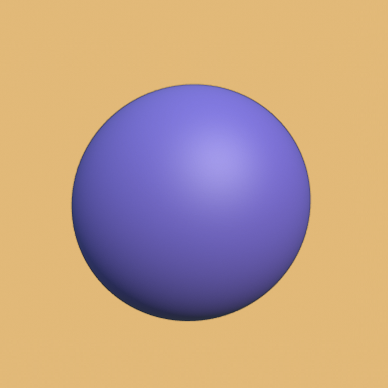
\includegraphics[width=0.3\linewidth ]{images/3d-9}
	}
	
	\caption[三维剪切流场测试结果]{$T=3,r_{\mathsf{tiny}}=0.01,h_L=1/128$时,三维变形流场的测试结果图.
		$(n_v,v_t)$在$T=0, \frac{T}{2}, T$时刻的值分别是$(16386,26624)$,$(266954,533904)$和$(107012,214020).$,
		$t=T$时刻的$E_{\infty}=3.03e-04,E_{\mathrm{vol}}=1.12e-06$.}
	\label{fig:3Dflow}
\end{figure}